\begin{figure}[htbp]
\centering
\resizebox{\textwidth}{!}{%
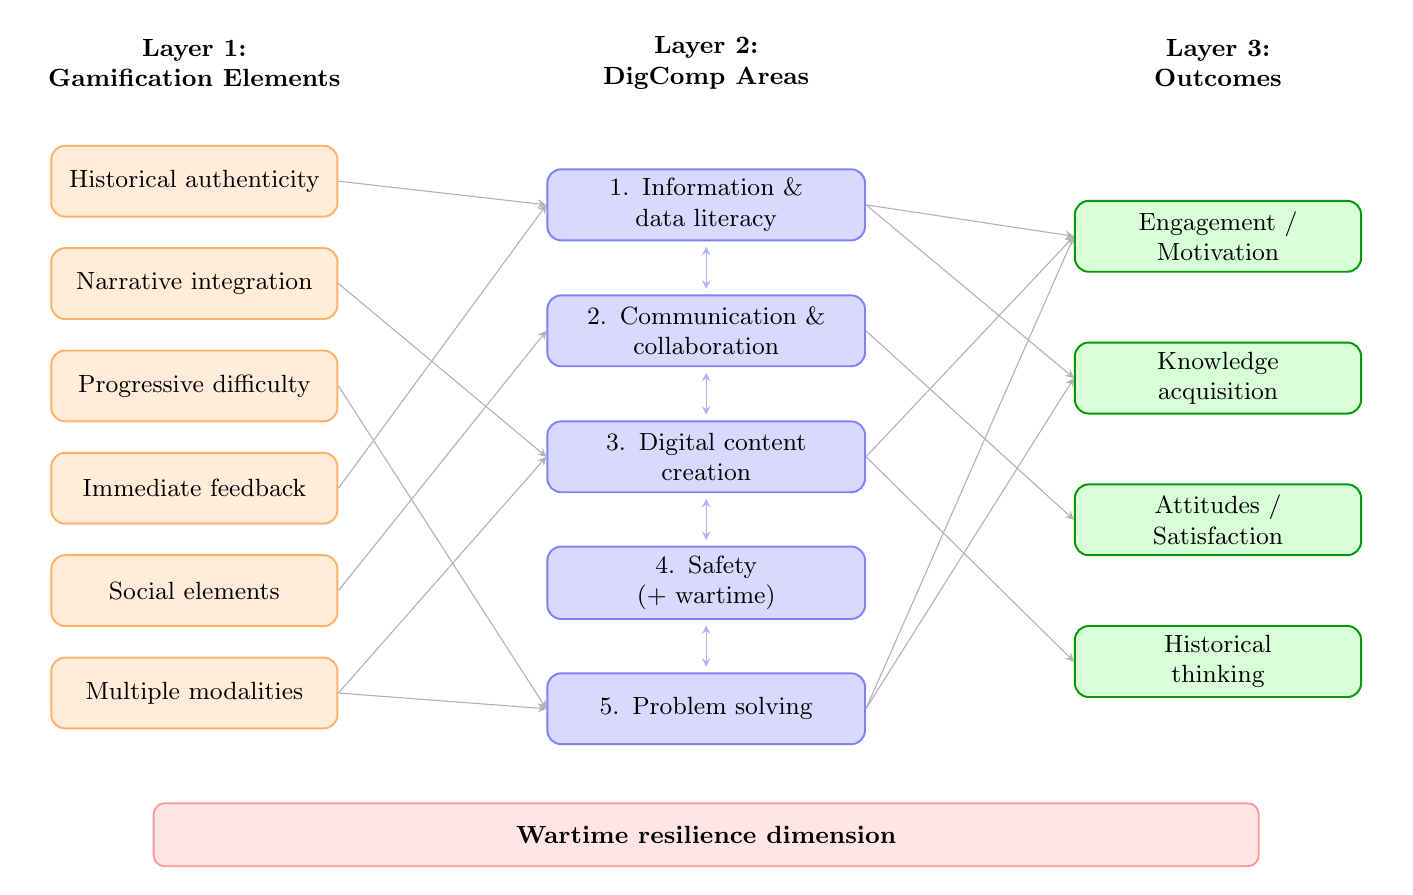
\begin{tikzpicture}[
  % Node styles
  gambox/.style={rectangle, rounded corners=5pt, draw=orange!60, fill=orange!15,
    text width=3.4cm, minimum height=0.9cm, align=center, font=\small,
    line width=0.7pt},
  dcbox/.style={rectangle, rounded corners=5pt, draw=blue!50, fill=blue!15,
    text width=3.8cm, minimum height=0.9cm, align=center, font=\small,
    line width=0.7pt},
  outbox/.style={rectangle, rounded corners=5pt, draw=green!60!black, fill=green!15,
    text width=3.4cm, minimum height=0.9cm, align=center, font=\small,
    line width=0.7pt},
  colhead/.style={font=\bfseries\small, align=center, text width=4cm},
  arr/.style={-stealth, draw=gray!60, thin},
]

% === Column positions ===
\def\colA{0}
\def\colB{6.5}
\def\colC{13}

% === Column headers ===
\node[colhead] (h1) at (\colA, 0) {Layer~1:\\Gamification Elements};
\node[colhead] (h2) at (\colB, 0) {Layer~2:\\DigComp Areas};
\node[colhead] (h3) at (\colC, 0) {Layer~3:\\Outcomes};

% === Layer 1: Gamification Elements (left, orange) ===
\node[gambox] (g1) at (\colA, -1.5) {Historical authenticity};
\node[gambox] (g2) at (\colA, -2.8) {Narrative integration};
\node[gambox] (g3) at (\colA, -4.1) {Progressive difficulty};
\node[gambox] (g4) at (\colA, -5.4) {Immediate feedback};
\node[gambox] (g5) at (\colA, -6.7) {Social elements};
\node[gambox] (g6) at (\colA, -8.0) {Multiple modalities};

% === Layer 2: DigComp Areas (center, blue) ===
\node[dcbox] (d1) at (\colB, -1.8) {1. Information \&\\data literacy};
\node[dcbox] (d2) at (\colB, -3.4) {2. Communication \&\\collaboration};
\node[dcbox] (d3) at (\colB, -5.0) {3. Digital content\\creation};
\node[dcbox] (d4) at (\colB, -6.6) {4. Safety\\(+ wartime)};
\node[dcbox] (d5) at (\colB, -8.2) {5. Problem solving};

% === Layer 3: Outcomes (right, green) ===
\node[outbox] (o1) at (\colC, -2.2) {Engagement /\\Motivation};
\node[outbox] (o2) at (\colC, -4.0) {Knowledge\\acquisition};
\node[outbox] (o3) at (\colC, -5.8) {Attitudes /\\Satisfaction};
\node[outbox] (o4) at (\colC, -7.6) {Historical\\thinking};

% === Arrows: Layer 1 → Layer 2 ===
% Historical authenticity → Area 1
\draw[arr] (g1.east) -- (d1.west);
% Narrative integration → Area 3
\draw[arr] (g2.east) -- (d3.west);
% Progressive difficulty → Area 5
\draw[arr] (g3.east) -- (d5.west);
% Immediate feedback → Area 1
\draw[arr] (g4.east) -- (d1.west);
% Social elements → Area 2
\draw[arr] (g5.east) -- (d2.west);
% Multiple modalities → Area 3
\draw[arr] (g6.east) -- (d3.west);
% Multiple modalities → Area 5
\draw[arr] (g6.east) -- (d5.west);

% === Arrows: Layer 2 → Layer 3 ===
% Area 1 → Knowledge acquisition
\draw[arr] (d1.east) -- (o2.west);
% Area 1 → Engagement
\draw[arr] (d1.east) -- (o1.west);
% Area 2 → Attitudes
\draw[arr] (d2.east) -- (o3.west);
% Area 3 → Historical thinking
\draw[arr] (d3.east) -- (o4.west);
% Area 3 → Engagement
\draw[arr] (d3.east) -- (o1.west);
% Area 5 → Knowledge acquisition
\draw[arr] (d5.east) -- (o2.west);
% Area 5 → Engagement
\draw[arr] (d5.east) -- (o1.west);

% === Bidirectional arrows: reciprocal competence development within Layer 2 ===
\draw[stealth-stealth, draw=blue!30, thin, shorten >=2pt, shorten <=2pt] (d1.south) -- (d2.north);
\draw[stealth-stealth, draw=blue!30, thin, shorten >=2pt, shorten <=2pt] (d2.south) -- (d3.north);
\draw[stealth-stealth, draw=blue!30, thin, shorten >=2pt, shorten <=2pt] (d3.south) -- (d4.north);
\draw[stealth-stealth, draw=blue!30, thin, shorten >=2pt, shorten <=2pt] (d4.south) -- (d5.north);

% === Bottom bar: Wartime resilience dimension ===
\node[rectangle, rounded corners=4pt, draw=red!40, fill=red!10,
  text width=13.8cm, minimum height=0.8cm, align=center,
  font=\small\bfseries, line width=0.7pt]
  (warbar) at ({\colB}, -9.8)
  {Wartime resilience dimension};

% Dashed lines from bottom bar to columns
\draw[dashed, draw=red!30, thin] (warbar.north -| \colA,0) -- (warbar.north -| \colA,0 |- g6.south);
\draw[dashed, draw=red!30, thin] (warbar.north -| \colB,0) -- (warbar.north -| \colB,0 |- d5.south);
\draw[dashed, draw=red!30, thin] (warbar.north -| \colC,0) -- (warbar.north -| \colC,0 |- o4.south);

\end{tikzpicture}%
}% end resizebox
\caption{Three-layer integration model for gamification-mediated digital competence development in history education. Layer~1 shows the six gamification design principles identified in the systematic review (Section~\ref{sec:gamification-review}). Layer~2 presents the five DigComp competence areas with history-specific interpretations (Section~\ref{sec:digcomp}). Layer~3 shows the outcome domains from the evidence gap map (Table~\ref{tab:evidence-gap-map}). Arrows indicate primary developmental pathways; the wartime resilience dimension (bottom) affects all three layers as a cross-cutting constraint. Bidirectional arrows between Layer~2 items reflect the reciprocal nature of competence development.}
\label{fig:gamification-digcomp-integration}
\end{figure}
